\documentclass[preprint]{sigplanconf}
\usepackage{xspace,url,subfigure,framed,amssymb,
            amsmath,mathpartir,hyperref,
            stmaryrd, graphicx, fancyvrb, stmaryrd % double brackets llbracket
}

\usepackage[T1]{fontenc}
\usepackage{beramono}
\usepackage{listings}
\usepackage[usenames,dvipsnames]{xcolor}

\lstdefinelanguage{Julia}%
  {morekeywords={abstract,break,case,catch,const,continue,do,else,elseif,%
      end,export,false,for,function,immutable,import,importall,if,in,%
      macro,module,otherwise,quote,return,switch,true,try,type,typealias,%
      using,while},%
   sensitive=true,%
   morecomment=[l]\#,%
   morecomment=[n]{\#=}{=\#},%
   morestring=[s]{"}{"},%
   morestring=[m]{'}{'},%
}[keywords,comments,strings]%

\lstset{%\lstinputlisting[language=Octave]{BitXorMatrix.m}
    language         = Julia,
    basicstyle       = \small\ttfamily,
    keywordstyle     = \bfseries\color{blue},
    stringstyle      = \color{magenta},
    commentstyle     = \color{ForestGreen},
    showstringspaces = false,
    stepnumber=1,
    numbers=left
}

\newcommand{\rn}[1]{#1}
\newcommand{\doi}[1]{doi:~\href{http://dx.doi.org/#1}{\Hurl{#1}}}

\newcommand{\xt}[1]{\texttt{#1}}

\newcommand{\OK}[1]{#1\;\text{OK}}
\newcommand{\abstype}[2]{\xt{abstract}~#1 <: #2}
\newcommand{\oftype}[2]{#1\,::\,#2}
\newcommand{\m}[2]{{#1}(#2)}
\newcommand{\contype}[2]{\xt{type}~#1 <: #2}
\newcommand{\any}{\xt{any}}
\newcommand{\jolt}{\xt{JOLT}}

\newcommand{\exact}[1]{{\llbracket #1 \rrbracket_{\xt{exact}}}}
\newcommand{\usable}[1]{{\llbracket #1 \rrbracket_{\xt{}}}}
\renewcommand{\ldots}{...}


\conferenceinfo{NOOL '16}{Month d--d, 20yy, City, ST, Country} 
\copyrightyear{20yy}
\copyrightdata{978-1-nnnn-nnnn-n/yy/mm}
\copyrightdoi{nnnnnnn.nnnnnnn}
\begin{document}
\title{Bottom-up Objects - Static Typing Without Types} 
\authorinfo{Benjamin Chung \and Paley Li \and Jan Vitek}{Northeastern University}{bchung@ccs.neu.edu \and \{pa.li,j.vitek\}@neu.edu} % Annon : Benjamin Chung, Jan Vitek}{Northeastern University}{}
\maketitle
% We should probably have some more introductory/motivational material herezies

\begin{abstract}
TODO:
\begin{itemize}
\item Julia has interesting inheritance mechanism, but it's completely dynamic.
\item What we purpose: using statically type check to allow more complex inheritance structure and bring static error messages for inheritance structure to Julia.
\item We formalised our ideas in JOLT, a minimal subset of Julia.
\end{itemize}
\end{abstract}


\begin{figure}
\centering
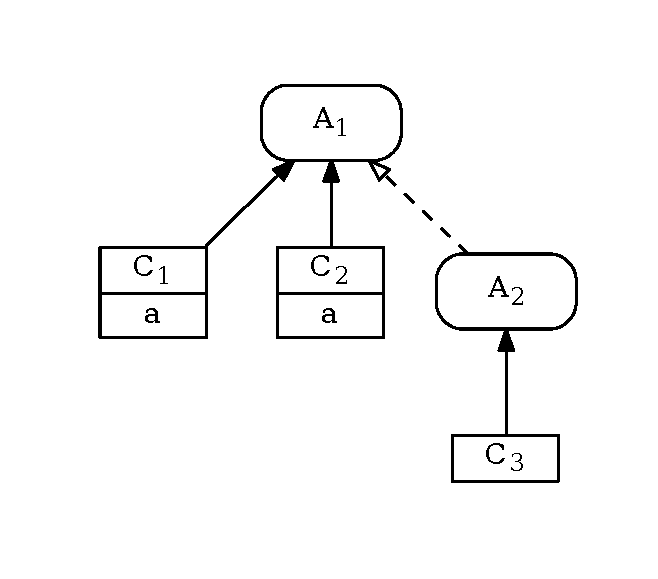
\includegraphics[scale=.6]{example2.pdf}
\caption{LALALALA}
\label{fig:algo}
\end{figure}

\section{Introduction}

Traditional typed object-oriented languages have a series of
common idioms: single dispatch, to figure out which method
to use in which situation, interfaces, to abstract over 
common means of access, and the means to statically
ensure that those interfaces are adhered to.

These practices are perfectly suitable for many contexts,
as is demonstrated by the success of langauges that have 
these features, but are not universally applicable, and
other languages that do not have any of these features
can use the object abstraction while retaining static 
safety.

In this paper, we will be talking about the Julia
programming language. Julia was originally designed
as a scientific computing language, in the vein of 
R or Matlab, and has a number of features designed
to support numeric computation and other tasks common
in scientific work.

\section{Julia}

From the perspective of object systems, Julia has several interesting features:
\begin{itemize}
\item Julia is \emph{dynamically typed}, and has no mechanism for statically
checking type correctness. However, as illustrated in figure~\ref{code:broken},
Julia code has many types.
\item The reason for all of these types is \emph{dispatch}. Julia provides 
full multimethod dispatch based on \emph{runtime type tags}, letting programmers
write code that is highly specified for a specific value.
\item However, one of the odder properties of this system is that Julia does not
allow explicit procedural interfaces, one of the key features of traditional 
object systems. Instead, Julia's interfaces, called \emph{abstract types}, 
define no explicit methods, relying on ``a collection of informal interfaces''
\cite{juliadocu} to abstract over implementations.
\end{itemize}

Figures~\ref{code:broken} and~\ref{fig:algo} show how these features can be used
in Julia code to provide for untyped object oriented programming. 

\begin{figure}

\lstinputlisting[language=Julia]{broken.jl}
\begin{Verbatim}[fontsize=\small]
ERROR: MethodError: no method matching example(::C3)
Closest candidates are:
  example(::C1)
\end{Verbatim}
\caption{Object inheritance in Julia}
\label{code:broken}
\end{figure}

\newpage

\begin{figure}
\begin{align*}
t ::=~& n ~|~ \any\\
d ::=~& \abstype{n}{t} ~|~ \contype{n}{t} \\
  & |~ \m{m}{\oftype{a}{t}, ~\ldots} = e\\
e ::=~& x ~|~ \xt{new} ~ n(e,~\ldots) ~|~ m(e,~\ldots) \\
\end{align*}
\caption{Static synatx of \jolt}
\label{fm:syntax}
\end{figure}

\jolt\space is a minimal formalism of a small subset of Julia. In figure~\ref{fm:syntax}, we present the synatx of \jolt.
Types (\xt{t}) in \jolt\space are either a name or the \any\space keyword. The expressions (\xt{e}) in \jolt\space only include varibles, 
object creation, and method invocation.

% \usable{A} \equiv \exact{A} \cup 
%	\bigcap_{C <: A} \usable{C} 
%	\bigcap_{A' <: A} \usable{A'}

\begin{figure}
\begin{mathpar}
\inferrule*[lab={\tiny TAbsSelf}]{ }{ \m{m}{\ldots, \oftype{a}{A}, \ldots} \in \usable{A} }

\inferrule*[lab={\tiny TConSelf}]{ }{ \m{m}{\ldots, \oftype{a}{C}, \ldots} \in \usable{C} }

\inferrule*[lab={\tiny TAbsChild}]{\forall\,C <: A: \m{m}{\ldots} \in \usable{C}\\ \forall\,A' <: A: \m{m}{\ldots} \in \usable{A'}}{ \m{m}{\ldots} \in \usable{A} }

\end{mathpar}
\caption{LALALA}
\end{figure}
\bibliographystyle{plain}
\bibliography{main}
\end{document}